\documentclass[conference]{IEEEtran}

%% keep it clean; only include those you need
\usepackage{amsfonts,amsmath,amssymb}
\usepackage{bbm}
\usepackage[inline]{enumitem}
\usepackage{graphicx}
\graphicspath{{./}{../image/}}
\usepackage[colorlinks=true,citecolor=blue,urlcolor=blue]{hyperref}
\usepackage[numbers]{natbib}
\usepackage{subcaption}
\usepackage{xcolor}


%% notations; only define those you use frequently
\newcommand{\EE}{{\mathbb{E}}}
\newcommand{\Fb}{\mathbf{F}}
\newcommand{\hb}{\mathbf{h}}
\newcommand{\Hc}{\mathcal{H}}
\newcommand{\Ib}{\mathbf{I}}
\newcommand{\Lc}{\mathcal{L}}
\newcommand{\PP}{{\mathbb{P}}}
\newcommand{\QQ}{{\mathbb{Q}}}
\newcommand{\xb}{\mathbf{x}}
\newcommand{\Oc}{\mathcal{O}}
\newcommand{\one}{\mathbbm{1}}
\newcommand{\Ocal}{\mathcal{O}}
\newcommand{\RR}{{\mathbb{R}}}
\newcommand{\XX}{{\mathbb{X}}}
\newcommand{\YY}{{\mathbb{Y}}}

\let\oldsubsubsection\subsubsection
\renewcommand{\subsubsection}[1]{\oldsubsubsection{\textbf{#1}}}

\let\proglang=\textsf
\let\pkg=\texttt

\newcommand{\sx}[1]{\textcolor{red}{(SX: #1)}}


\begin{document}


\title{\huge UNet-HCRF Integration for EEG Pattern Recognition}

\author{\IEEEauthorblockN{Xiaohang Ma}
\IEEEauthorblockA{\textit{Department of Mathematics} \\
\textit{University of Connecticut}\\
Storrs, CT, USA \\
xiaohang.ma@uconn.edu}
\and
\IEEEauthorblockN{Shiying Xiao}
\IEEEauthorblockA{\textit{Department of Statistics} \\
\textit{University of Connecticut}\\
Storrs, CT, USA \\
shiying.xiao@uconn.edu}
\and
\IEEEauthorblockN{Xiaohui Yin}
\IEEEauthorblockA{\textit{Department of Statistics} \\
\textit{University of Connecticut}\\
Storrs, CT, USA \\
xiaohui.yin@uconn.edu}
}

\maketitle


\begin{abstract}


%In this project, we will integrate powerful deep neural networks and
%statistical methods with a probabilistic graphical model (PGM) to effectively
%tackle sequence labeling tasks on a heterogeneous medical care dataset.


\end{abstract}


\begin{IEEEkeywords}


classification, probabilistic graphical model, spectrogram,
variational inference, wavelet transformation


\end{IEEEkeywords}


\section{Introduction}


Electroencephalography (EEG) pattern recognition plays a pivotal role in
various fields, including neuroscience, clinical medicine, and human-computer
interaction. By analyzing brain electrical activity, we can gain deeper
insights into brain states and functions, providing a scientific basis for
diagnosing and treating neurological disorders, as well as developing
brain-computer interfaces. EEG pattern recognition not only helps to unveil the
mechanisms of the brain but also enables the development of smarter and more
human-centric technologies. However, traditional manual analysis of EEG signals
is a time-consuming and subjective process, often leading to inconsistencies in
diagnosis~\citep{liu2013recognizing}.


In recent years, deep learning has emerged as a powerful tool to automate and
improve EEG pattern recognition~\citep{craik2019deep}. Neural network
architectures like convolutional neural network (CNN), long short-term memory
(LSTM) and Transformer models have revolutionized EEG data processing.
Additionally, hidden conditional random fields (HCRFs) have been employed for
modeling label dependencies, demonstrating promising results.
While these methods have shown individual strengths, a comprehensive
approach that leverages their complementary capabilities is essential for
tackling complex, multi-modal datasets.


This project introduces a novel framework that combines deep neural networks
and probabilistic graphical models (PGMs) to enhance the accuracy of EEG
pattern recognition . By employing UNet~\citep{ronneberger2015unet} for feature
extraction and integrating them with HCRF models, we aim to improve the
precision of EEG pattern recognition tagging. Furthermore, mean-field
approximation techniques are utilized for efficient inference, ensuring a
computationally efficient yet effective approach.
This integration of modern neural network architectures with HCRFs offers
a robust and promising solution for EEG pattern recognition tasks.


\section{Background}
%Background & Related Work: background info and literature survey.

\sx{Add UNet}

Deep neural networks, particularly recurrent neural networks (RNNs) like LSTM,
are widely used for sequence labeling due to their ability to capture
long-range dependencies in sequences. Bidirectional LSTM (Bi-LSTM) further
enhances this by processing sequences in both directions, improving context
understanding.
CRFs, on the other hand, are commonly used for structured predictions,
modeling dependencies between neighboring labels to ensure valid output
sequences.
\citet{huang2015bidirectional} pioneered the use of Bi-LSTM integrated with
CRFs for sequence labeling tasks, demonstrating their effectiveness in
extracting features and ensuring label consistency.


However, Bi-LSTMs can still struggle to fully account for structural
dependencies between predicted labels, leading to potential inconsistencies in
the output sequence. Additionally, they typically require large amounts of
labeled data and are computationally expensive, making them challenging to
deploy in resource-constrained environments, such as hospitals.


Transformer-based models, such as BERT~\citep{devlin2019bert},
have emerged as powerful alternatives to traditional RNN-based approaches.
Trained on massive datasets in an unsupervised manner, Transformer can be
fine-tuned for various natural language processing tasks,
including sequence labeling.
\citet{devlin2019bert} directly compared BERT to traditional models, including
Bi-LSTM, and demonstrated its superior performance on tasks like named entity
recognition, highlighting its ability to capture more feature information
than LSTM models.


While CRFs are effective for modeling label dependencies, they often lack
efficient closed-form solutions, especially for complex models beyond
linear-chain CRFs. To address this, \citet{krahenbuhl2011efficient} introduced
the use of mean-field approximation to solve more general CRFs in the context
of complex prediction tasks. By minimizing the Kullback-Leibler (KL)
divergence, mean-field approximation can be reduced to a fixed-point iteration,
providing a faster and more efficient approach for training and inference
while maintaining suitable accuracy. \citet{zheng2015conditional} further
extended this technique by reformulating mean-field approximation for fully
connected CRFs, integrating an RNN structure to capture temporal dependencies.


\section{Methods}


We begin by introducing the necessary notations.
Let $\xb = (x_0, x_1, \dots, x_N)^\top$ represent the feature vector of the
input image, where $x_0$ denotes the global feature capturing overall image
characteristics, and $x_i$ ($1 \leq i \leq N$) corresponds to a local feature
extracted from the $i$-th pixel. Here, $N$ denotes the total number of pixels
in the image. Let $y \in Y$ represent the class label associated with the image,
where $Y$ is a finite set containing $\vert Y \vert$ possible class labels.
For any feature $\xb$, a corresponding vector of unobserved variables, referred
to as hidden part states and denoted by $\hb = (h_1, \dots, h_N)^\top$,
is introduced. Each $h_i \in H$ represents the hidden part state associated
with $x_i$ for $i = 1, \dots, N$. Here, $H$ is a finite set of hidden part
states, and $\vert H \vert$ denotes the cardinality of this set.


\subsection{CNN-HCRF Model}


Following the theory of random fields as outlined
by~\citet{quattoni2004conditional} and~\citet{wang2006hidden},
given the feature $\xb$, its corresponding hidden part states $\hb$,
and the class label $y$, a hidden conditional random field (HCRF) can be
expressed in exponential form as follows:
\begin{equation}
\label{eq:hcrf}
\PP(y, \hb \mid \xb; \theta)
= \frac{\exp\left(\Phi(y, \hb, \xb; \theta)\right)}
{\sum_{y^\prime \in Y} \sum_{\hb \in H^N}
\exp\left(\Phi(y^\prime, \hb, \xb; \theta)\right)},
\end{equation}
where $\theta$ is the parameter of the model,
$H^N$ denotes the set of all possible hidden part states of $N$ hidden parts,
and $\Phi(y, \hb, \xb; \theta) \in \RR$ refers to a potential function
depending on the feature $\xb$ and parameterized by $\theta$.


From Equation~\ref{eq:hcrf}, the probability of class label $y$ for the given
feature $\xb$ is:
\begin{equation*}
\begin{split}
\PP(y \vert \xb; \theta) &= \sum_{\hb \in H^N} \PP(y, \hb \mid \xb; \theta) \\
&= \frac{\sum_{\hb \in H^N} \exp\left(\Phi(y, \hb, \xb; \theta)\right)}
{\sum_{y^\prime \in Y} \sum_{\hb \in H^N}
\exp\left(\Phi(y^\prime, \hb, \xb; \theta)\right)}.
\end{split}
\end{equation*}


The potential of the HCRF model, $\Phi(y, \hb, \xb; \theta)$, is defined in the
following form:
\begin{align*}
\Phi(y, \hb, \xb; \theta) &= \underbrace{
\sum_{j \in \nu} \phi(h_j, x_j; \omega) +
\sum_{i \neq j} \psi(h_i, h_j, x_i, x_j; \eta)}_{
% \propto \log \PP( \hb \vert \xb; \theta)
\textrm{Measures log-likelihood $\log \PP(\hb \vert \xb; \theta)$}} \\
& + \underbrace{
\sum_{j \in \nu} \varphi(y, h_j, x_j; \delta) + \vartheta(y, x_0; \varpi)}_{
% \propto \log \PP(y | \hb, \xb; \theta)
\textrm{Measures log-likelihood $\log \PP(y \vert \hb, \xb; \theta)$}},
\end{align*}
where the detailed components are described below.


\textbf{Unary potential} $\phi(h_j, x_j; \omega)$ measures the likelihood of
the local feature $x_j$ is assigned as the hidden attention state $h_j$.
The parameter $\omega$ is learned through the end-to-end CNN-UNet training
structure. This likelihood is computed by applying a softmax operation to the
feature maps produced by the CNN.


\textbf{Binary potential} $\psi(h_i, h_j, x_i, x_j; \eta)$ balances the
hidden label compatibility of the neighboring pixels on the feature $\xb$.
The potential is defined through a common contrast-sensitive two-kernal
potentials~\citep{krahenbuhl2011efficient, chen2022end}:
\begin{equation*}
\begin{split}
& \psi(h_i, h_j, x_i, x_j; \eta) = \mu(h_i, h_j) \Bigg[
\omega_1 \exp \bigg(
-\frac{\left\lvert p_i - p_j \right\rvert^2}{2\eta_\alpha^2} \\
&\quad
- \frac{\left\lvert x_i - x_j\right\rvert^2}{2\eta_\beta^2}
\bigg) + \omega_2 \exp \left(
- \frac{\left\lvert p_i - p_j \right\rvert^2}{2 \eta_\gamma^2}
\right)
\Bigg],
\end{split}
\end{equation*}
where $\mu(h_i, h_j)$ is a label compatibility function that describes
the interactive influences between different pairs of classes,
and $p$ refers to the pixel position.
The parameters $\omega_1$ and $\omega_2$ serve as linear combination weights,
controlling the contributions of the first and second kernels, respectively.
And the parameters $\eta_\alpha$, $\eta_\beta$ and $\eta_\gamma$ control the
influence of the corresponding feature spaces.


\textbf{Unary potential} $\varphi(y, h_j; \delta)$ measures the compatibility
between global class label $y$ and the hidden local state $h_j$.
This potential is parametrized as:
\begin{equation*}
\varphi(y, h_{j}; \delta) = \sum_{a \in Y} \sum_{b \in H} \delta_{a, b}
\cdot \one(y = a) \cdot \one(h_j = b).
\end{equation*}
where $\one(\cdot)$ is an indicator function, and $\delta_{a,b}$ denotes the
likelihood of class label $y = a$ containing a joint with hidden state
$h_j = b$, which is learned during training.


\textbf{Global potential} $\vartheta(y, x_0; \varpi)$ measures the likelihood of
the global feature $x_0$ is assigned as the class label $y$, where the parameter
$\varpi$ is learned during training process.


\subsection{Variational Inference of HCRF}


The inclusion of the hidden variable $\hb$ enhances the interpretability of the
model. However, training the model using maximum likelihood estimation
necessitates the calculation of the summation
$\sum_{\hb \in H^N} \PP(y, \hb \mid \xb; \theta)$, and the presence of the
hidden variable renders the exact computation of this summation intractable.
To circumvent this challenge, a mean-field variational inference framework is
employed, enabling efficient estimation of the log-likelihood
$\log \PP(y \mid \xb; \theta)$.


\subsubsection{ELBO Under Mean-Filed Variational Family}


The mean-field varepsilon family approximation of
$\log \PP(\hb \mid y, \xb; \theta)$ is given by:
\begin{equation*}
\QQ(\hb) = \prod_{i=1}^N q_i(h_i),
\end{equation*}
where $q_i(h_i)$ represents the approximate distribution of the individual
hidden variable.


Under the mean-field family, the evidence lower bound (ELBO) is given by
\begin{equation}
\begin{split}
& \Lc(\QQ) = \EE_{\QQ(\hb)} \log\PP(y, \hb \mid \xb; \theta)
- \EE_{\QQ(\hb)} \log q(\hb) \\
&\quad = \sum_{i=1}^N \EE_{q_i(h_i)}
\left[ \phi(h_j, x_j; \omega) + \varphi(y, h_j, x_j; \delta) \right] \\
&\quad + \sum_{i=1}^N \sum_{j=1}^N \sum_{l,l^\prime} \one_{\{i \neq j\}} 
\QQ(h_i = l) \QQ(h_j = l^\prime) \mu(l, l^\prime) \\
&\quad \Bigg[ \omega_1 \exp \left(
- \frac{\left\lvert p_i - p_j \right\rvert^2}{2\eta_\alpha^2}
- \frac{\left\lvert x_i - x_j \right\rvert^2}{2\eta_\beta^2} \right) \\
&\quad + \omega_2 \exp \left(
- \frac{\left\lvert p_i - p_j \right\rvert^2}{2\eta_\gamma^2}
\right) \Bigg] \\
&\quad - \sum_{i=1}^N \EE_{q_i} \log q_i(h_i) + \vartheta(y, x_0; \varpi).
\end{split}
\end{equation}


\begin{figure*}[tbp]
\centering
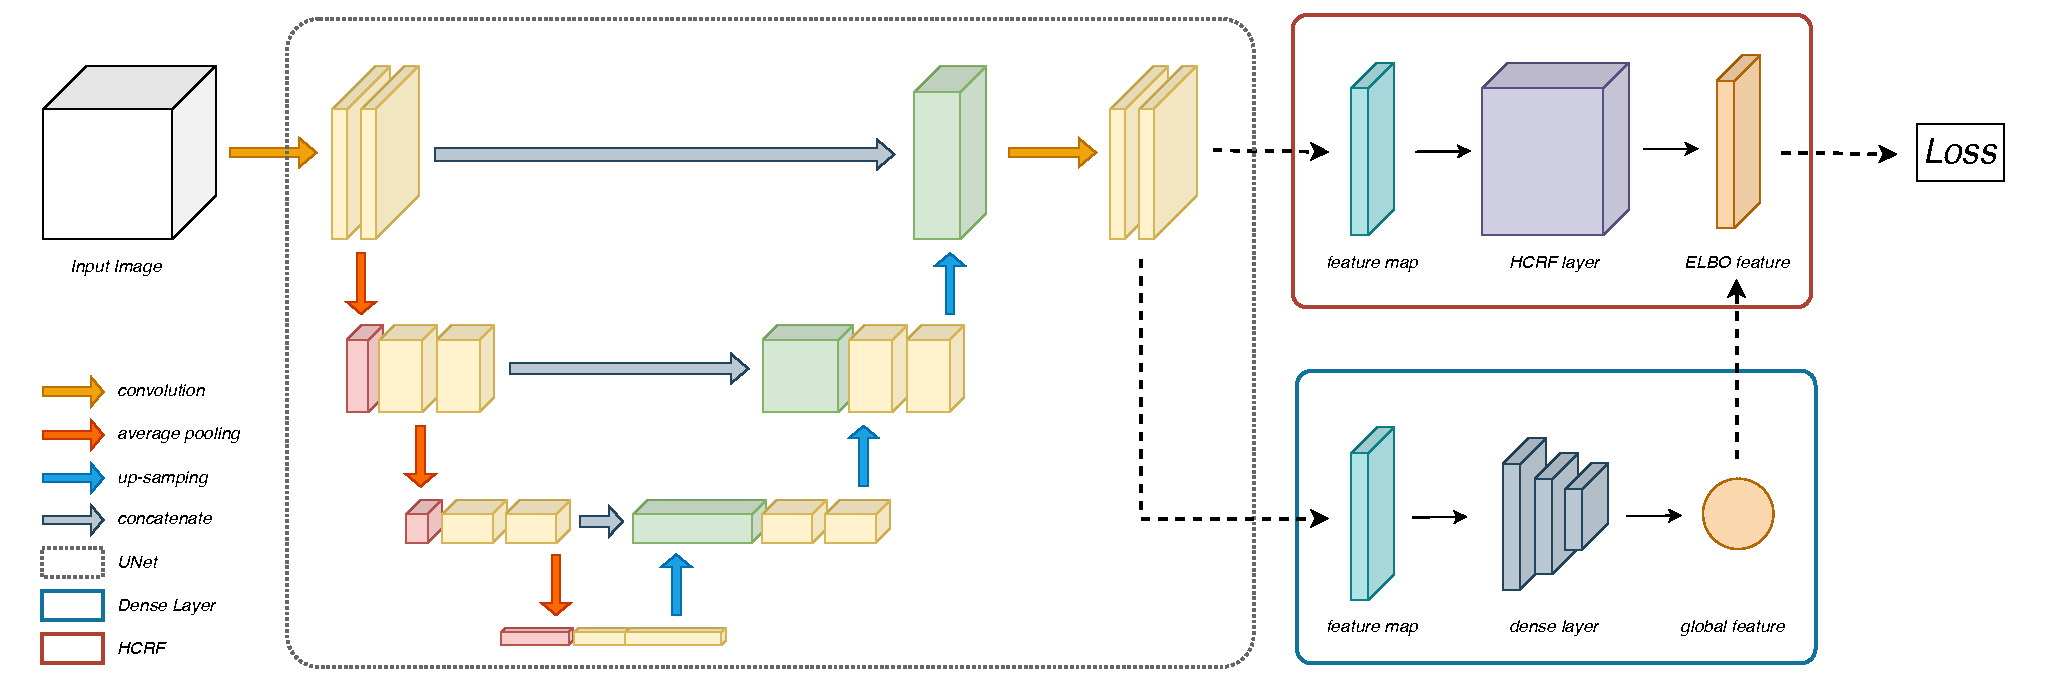
\includegraphics[width=\textwidth]{workframe}
\caption{\sx{caption}.}
\label{fig:workframe}
\end{figure*}


\subsubsection{Updating Variational Family}


By employing the coordinate ascent variational inference (CAVI) algorithm,
an efficient method for approximating posterior distributions in probabilistic
models, the optimization process involves iteratively updating each variational
factor while holding others fixed. Specifically, fixing $q_j(h_j)$,
$\forall j \neq i$, the optimal $q_i(h_i)$ that maximizes $\Lc(q_i(h_i))$
is computed as:
\begin{equation*}
\QQ(h_i) \propto \exp\{\EE_{\QQ(\hb_{-i})}
\log\PP(y, h_i, \hb_{-i} \mid \xb; \theta)\}.
\end{equation*}
Thus, we can get that
\begin{equation*}
\begin{split}
q_i(l) &= \frac{1}{Z_i} \exp \Bigg\{
\phi(h_j, x_j; \omega) + \varphi(y, h_j, x_j; \delta) \\
&+ \sum_{j \neq i} \sum_{l^\prime} q(l^\prime) \mu(l, l^\prime) 
\Bigg[ \omega_1 \exp \bigg(
- \frac{\left\lvert p_i - p_j \right\rvert^2}{2\eta_\alpha^2}\\
&- \frac{\left\lvert x_i - x_j \right\rvert^2}{2\eta_\beta^2}
\bigg)
+ \omega_2 \exp \left(
- \frac{\left\lvert p_i - p_j 
\right\rvert^2}{2\eta_\gamma^2}
\right)
\Bigg]
\Bigg\},
\end{split}
\end{equation*}
where $Z_i$ is the normalizing constant.


\subsubsection{Computational Complexity Analysis}


\paragraph{Updating variational family}


The computationally intensive step in the fixed-point iteration of $q_i(h_i)$
is the message passing process, which involves convolving $\QQ(\hb)$ with a
Gaussian kernel within the binary potential $\psi(h_i, h_j, x_i, x_j; \eta)$.
This operation requires $\Oc(N^2)$ runtime for $N$ pixels when evaluated
exactly. To improve computational efficiency, a truncated Gaussian kernel is
utilized, which is supported only within a specific proportion of the
untruncated standard deviation. This approximation reduces the complexity of 
message passing to linear time, $\Oc(N)$.


\paragraph{Computation of the ELBO}


The summation over the product of $q_i(h_i)q_j(h_j)$ and the Gaussian kernel
in $\psi(h_i, h_j, x_i, x_j; \eta)$ also incurs a time complexity of $\Oc(N^2)$.
By applying a similar truncated Gaussian kernel approximation, the runtime can
be reduced to $\Oc(N)$.


\section{Experiment Details}


\subsection{Dataset Description}


The dataset used in this research is the Harmful Brain Activity Classification
(HMS) dataset~\citep{jing2023development}, provided by Harvard Medical School
for research purposes. This dataset comprises EEG recordings and their
corresponding spectrograms, segmented into 50-second-long samples derived from
10-minute windows of brain activity.
The longer 10-minute window allows for the model to pick up on further insights
regarding the nature of the brain activity. Each EEG sample, representing 50
seconds of brain activity measured by 19 scalp electrodes, is paired with a
matching spectrogram.
The EEG samples were labeled by expert annotators from Critical Care EEG
Monitoring Research Consortium (CCEMRC) into one of six types of brain
activity: seizures, generalized periodic discharges (GPD), lateralized
periodic discharges (LPD), lateralized rhythmic delta activity (LRDA),
generalized rhythmic delta activity (GRDA), and other.


Expert agreement was high for some segments; nevertheless, instances of
disagreement were observed. The segments were categorized as follows:
\begin{enumerate*}[label = (\roman*)]
\item ``Idealized'': Segments with high levels of expert agreement.
\item ``Proto'': Segments where approximately half of the experts labeled them
as ``other'', while the other half assigned one of the remaining five labels.
\item ``edge'': Segments where experts were roughly split between two of the
five named patterns.
\end{enumerate*}
Figure~\ref{fig:ex} shows an example of EEG patterns with different level of
agreement.


\begin{figure}[tbp]
\centering
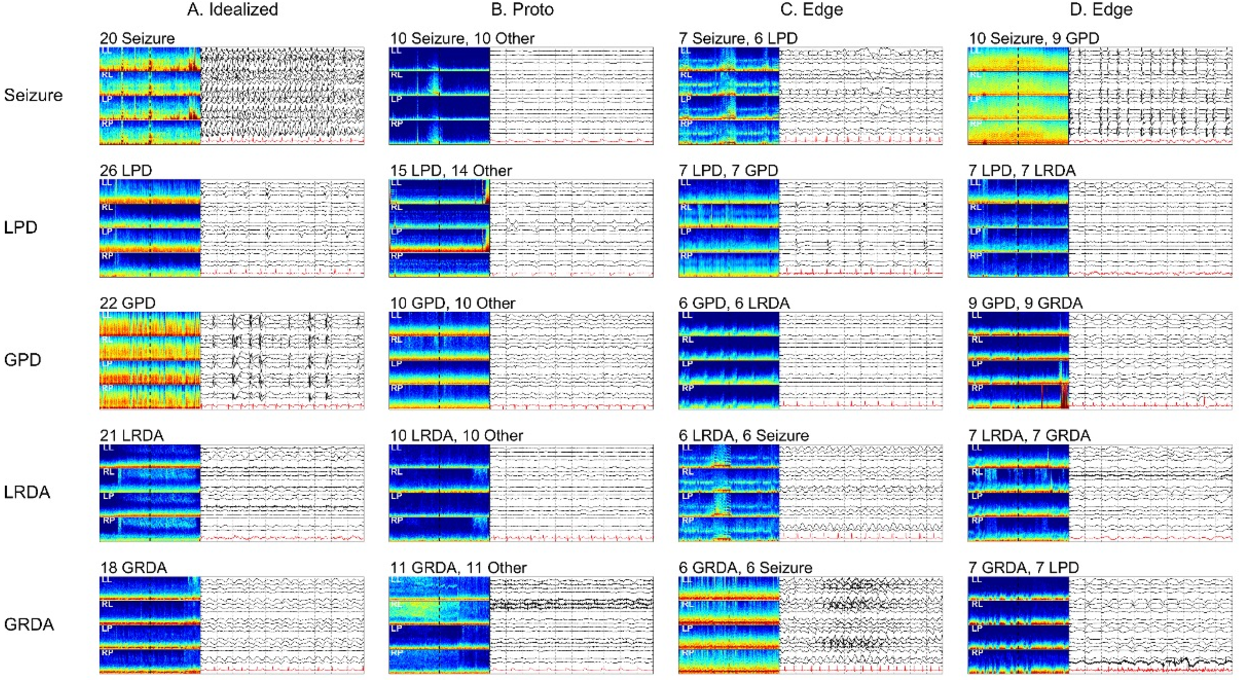
\includegraphics[width=.48\textwidth]{example}
\caption{Examples of EEG patterns with different levels of expert agreement,
sourced from the HMS dataset.}
\label{fig:ex}
\end{figure}


\subsection{Data Preparation}


The data preparation process involves multiple steps to extract spectrogram
features from EEG data, enhance signal quality, and ensure the features are
appropriately scaled and normalized for analysis.


\textbf{Wavelet denoising}: EEG signals were denoised using wavelet
transformation to improve signal quality by decomposing the signal into wavelet
coefficients, applying thresholding to remove noise, and reconstructing the
denoised signal.
%via \pkg{pywt} \proglang{Python} package


\textbf{Feature Extraction}: A bipolar montage technique is applied to the
denoised EEG signals to calculate the difference between adjacent electrode
signals, generating four representative montage features from the original 19
features. Figure~\ref{fig:inion} illustrates the bipolar electrode chains used
in this study.


\textbf{Spectrogram transformation}: The denoised EEG signals are converted
into Mel-spectrograms, which are log-transformed to enhance spectral
information and compress the dynamic range. Figure~\ref{fig:EEG} shows an
example of the denoised EEG signal and its corresponding transformated
spectrogram.
%using the \pkg{librosa} \proglang{Python} package


\textbf{Normalizatio}n: The Mel-spectrogram values are standardized to a range
of $[-1,1]$ to ensure consistent feature scaling and facilitate model training.


\textbf{Imputation}: Missing values in the data are imputed with the mean of
non-missing values within each spectrogram. If all values are missing,
the spectrogram is set to zero to maintain data consistency.


\begin{figure}[tbp]
\centering
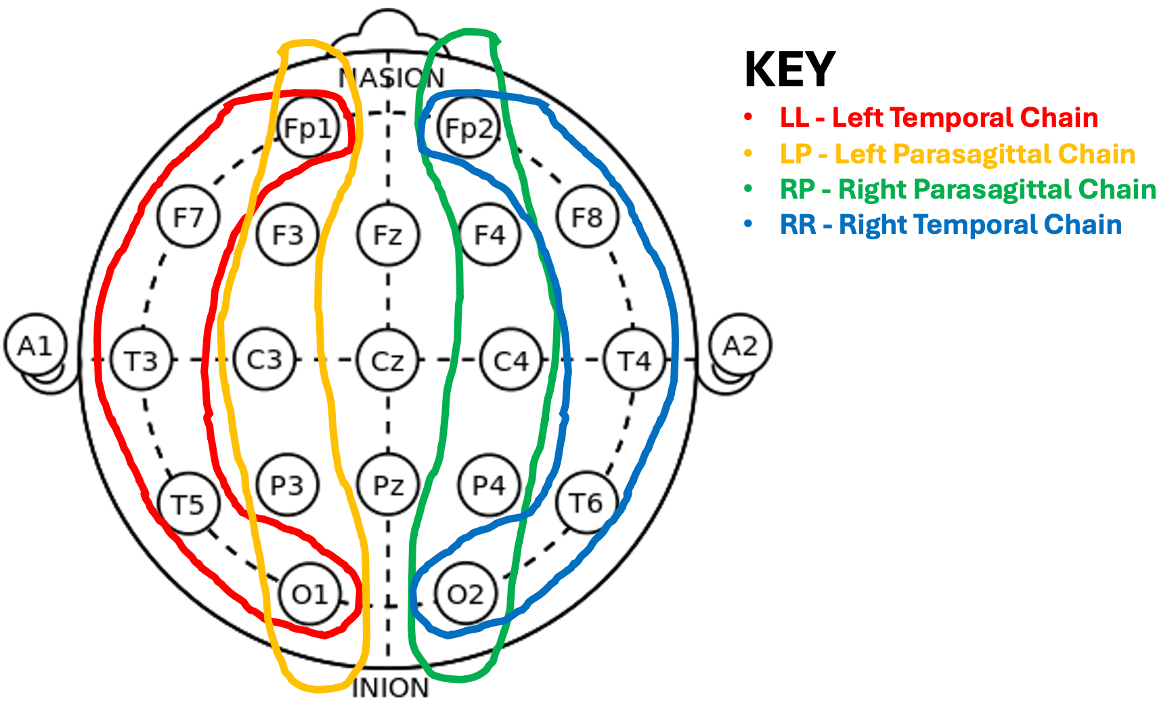
\includegraphics[width=.45\textwidth]{inion}
\caption{Chains employed to determine representative montage features via
a bipolar montage, sourced from Kaggle.}
\label{fig:inion}
\end{figure}


\begin{figure}
\centering
\begin{subfigure}[b]{0.45\textwidth}
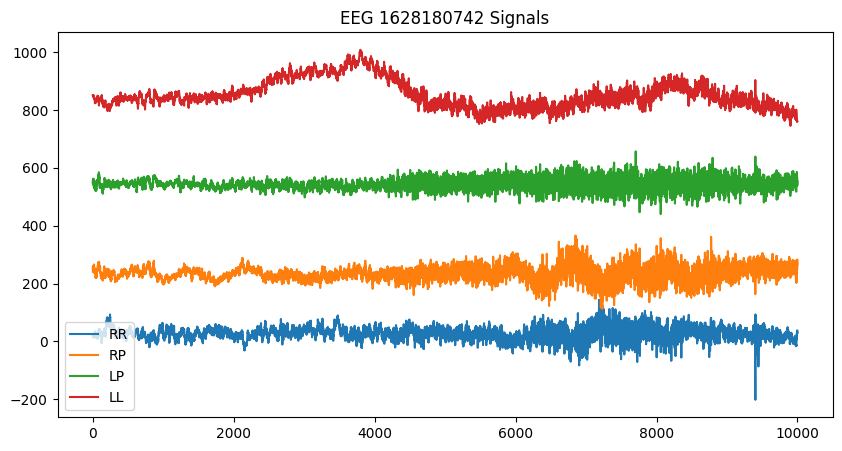
\includegraphics[width=\textwidth]{EEG_Signal}
\end{subfigure}
\hfill
\begin{subfigure}[b]{0.45\textwidth}
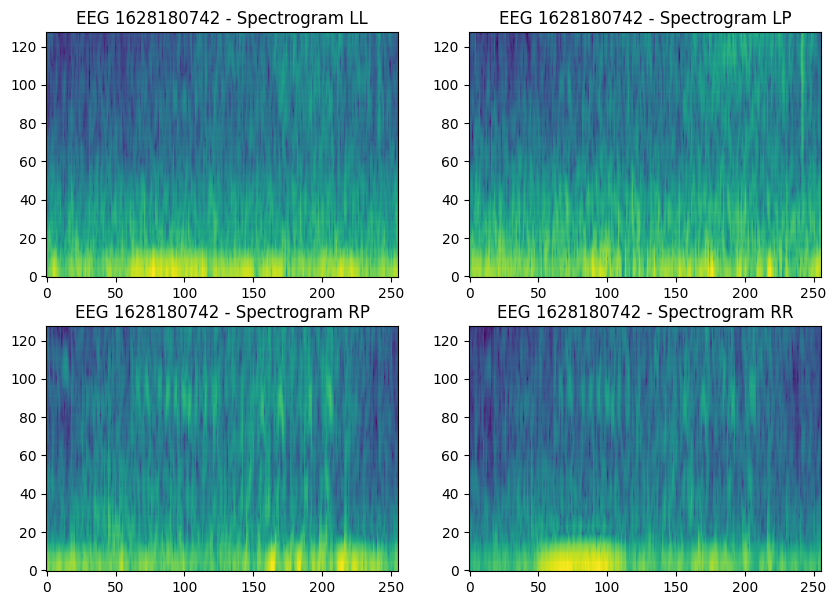
\includegraphics[width=\textwidth]{EEG_Spectrogram}
\end{subfigure}
\caption{An example of the denoised EEG signal (top) and its corresponding
spectrogram representation (bottom).}
\label{fig:EEG}
\end{figure}


\subsection{Loss Function}


The model outputs an array of predicted probabilities for each label class.
To evaluate its performance, the Kullback-Leibler (KL) divergence metric is
employed. This metric is suitable for comparing two probability distributions: 
the ground truth probability distribution $\XX$ and the predicted probability
distribution $\YY$. The KL divergence between these two distributions is
defined as:
\begin{equation*}
D_\mathrm{KL}(\XX \Vert \YY) = \sum \XX \log\left(\frac{\XX}{\YY}\right)
\end{equation*}


The KL divergence offers the advantage of direct applicability as a loss
function during model training, eliminating the need for an alternative loss
function. Its differentiability enables efficient gradient-based optimization
techniques.


\subsection{Learning Rate Scheduler}


To optimize the model's training process, a cosine annealing learning rate
scheduler was employed. This technique ensures a smooth and gradual decrease in
the learning rate, preventing abrupt changes that can destabilize the training
process. By allowing the model to explore a wider parameter space initially and
then refining its solution towards the end, cosine annealing contributes to
better convergence and reduced oscillations in the loss function.


As depicted in Figure~\ref{fig:cos}, the learning rate for both the pre-trained
UNet and the fine-tuned HCRF exhibit a similar pattern. Both start with a
relatively high learning rate, which gradually decreases over time.
This smooth decay helps ensure stable training and optimal convergence.


\begin{figure}
\centering
\begin{subfigure}[b]{0.45\textwidth}
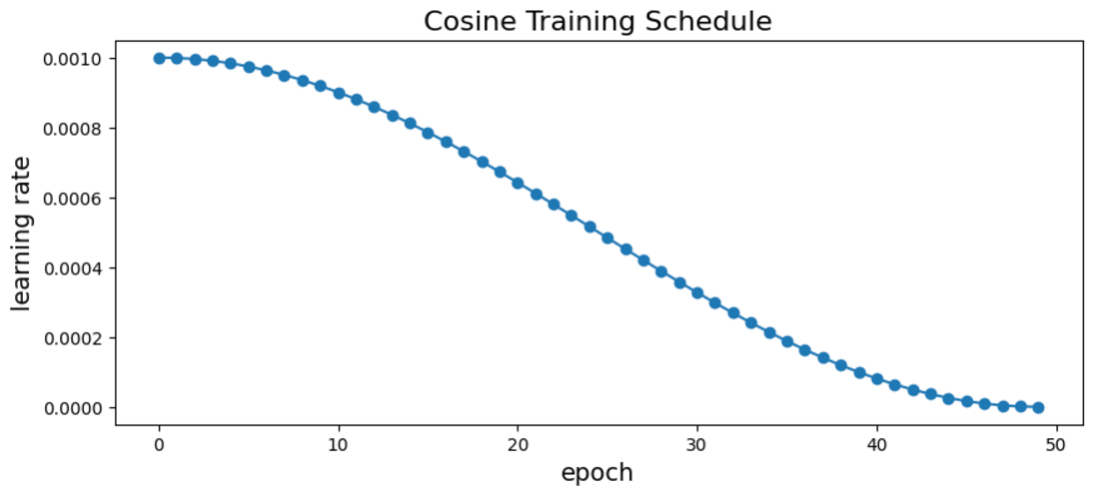
\includegraphics[width=\textwidth]{pretrain}
\end{subfigure}
\hfill
\begin{subfigure}[b]{0.45\textwidth}
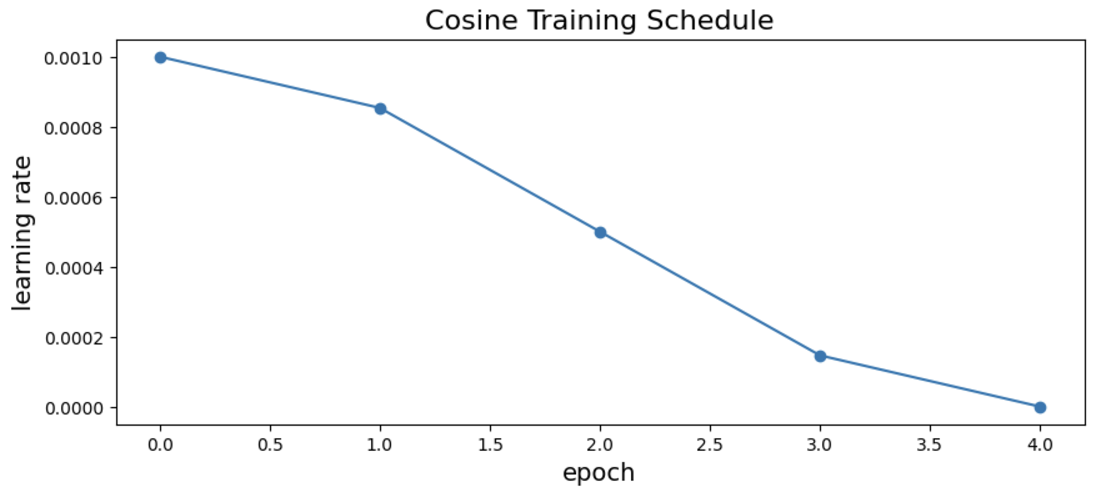
\includegraphics[width=\textwidth]{finetune}
\end{subfigure}
\caption{The learning rate schedulers for the pre-trained UNet (top) and
the fine-tuned HCRF (bottom).}
\label{fig:cos}
\end{figure}


\section{Results}


\section{Conclusion}


\bibliographystyle{IEEEtranN}
\bibliography{refs}

\end{document}
